\documentclass{article}

\usepackage[utf8]{inputenc}
\usepackage[T1]{fontenc}
% \usepackage[french]{babel}
\usepackage{amssymb}
\usepackage{ntheorem}
\usepackage{amsmath}
\usepackage{amssymb}
\usepackage[ a4paper, hmargin={3cm, 3cm}, vmargin={3cm, 3cm}]{geometry}

\usepackage{hyperref}
\hypersetup{
    colorlinks,
    citecolor=black,
    filecolor=black,
    linkcolor=blue,
    urlcolor=blue
}

\theoremstyle{plain}
\theorembodyfont{\normalfont}
\theoremseparator{~--}
\newtheorem*{define}{Définition}%[section]

\usepackage{tikz}
\usetikzlibrary{automata, positioning, arrows}
\usepackage{capt-of}

\title{Algorithme avancé}
\author{Valeran MAYTIE}
\date{}

\begin{document}
  \maketitle{}

  mail : \href{mailto:marc-atoine.weisserc@centralsupelec.fr}
              {marc-atoine.weisserc@centralsupelec.fr}

  \tableofcontents{}

  \section{NP-Complétude}

    \subsection{Séquençage ADN}
    
      Recomposition de séquence ADN
      Le but est de concaténer, dans le bon ordre, les différents fragments
      d'ADN afin de reconstituer le fragment d'ADN

      \underline{Contraintes} :
      \begin{itemize}
        \item La terminaison de chaque fragment doit être compatible
              avec le commencement du suivant.

        \item Chaque fragment doit apparaitre une et une seule fois.
      \end{itemize}

      Problème compliqué, explose le temps de calcul

    \subsection{Sir Hamilton}

      \subsubsection{Le voyage fermé autour du monde} \vspace{5mm}
  
      \begin{center}
      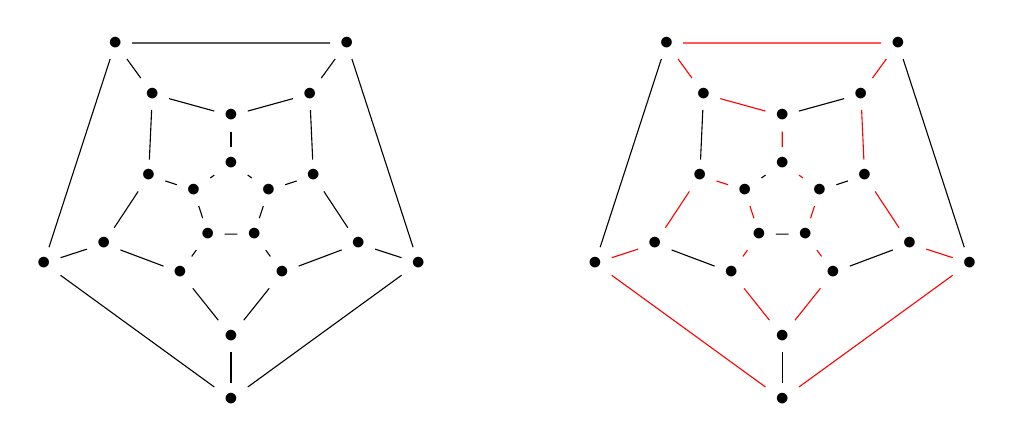
\begin{tikzpicture}
        \node (a) at (270:2.5) {$\bullet$};
        \node (b) at (342:2.5) {$\bullet$};
        \node (c) at (54: 2.5)  {$\bullet$};
        \node (d) at (126:2.5) {$\bullet$};
        \node (e) at (198:2.5) {$\bullet$};

        \node (g) at (270:1.7) {$\bullet$};
        \node (h) at (342:1.7) {$\bullet$};
        \node (i) at (54: 1.7) {$\bullet$};
        \node (j) at (126:1.7) {$\bullet$};
        \node (k) at (198:1.7) {$\bullet$};

        \node (a') at (90: 0.5) {$\bullet$};
        \node (b') at (162:0.5) {$\bullet$};
        \node (c') at (234:0.5)  {$\bullet$};
        \node (d') at (306:0.5) {$\bullet$};
        \node (e') at (378:0.5) {$\bullet$};

        \node (g') at (90: 1.1) {$\bullet$};
        \node (h') at (162:1.1) {$\bullet$};
        \node (i') at (234:1.1)  {$\bullet$};
        \node (j') at (306:1.1) {$\bullet$};
        \node (k') at (378:1.1) {$\bullet$};

        \draw (a) -- (b) -- (c) -- (d) -- (e) -- (a);
        \draw (a') -- (b') -- (c') -- (d') -- (e') -- (a');
        \draw (a) -- (g);
        \draw (b) -- (h);
        \draw (c) -- (i);
        \draw (d) -- (j);
        \draw (e) -- (k);

        \draw (a') -- (g');
        \draw (b') -- (h');
        \draw (c') -- (i');
        \draw (d') -- (j');
        \draw (e') -- (k');

        \draw (g) -- (j') -- (h) -- (k') -- (i) -- (g') -- (j) -- (h') -- (k)
              -- (i') -- (g);

        \begin{scope}[xshift=7cm]

        \node (a) at (270:2.5) {$\bullet$};
        \node (b) at (342:2.5) {$\bullet$};
        \node (c) at (54: 2.5)  {$\bullet$};
        \node (d) at (126:2.5) {$\bullet$};
        \node (e) at (198:2.5) {$\bullet$};

        \node (g) at (270:1.7) {$\bullet$};
        \node (h) at (342:1.7) {$\bullet$};
        \node (i) at (54: 1.7) {$\bullet$};
        \node (j) at (126:1.7) {$\bullet$};
        \node (k) at (198:1.7) {$\bullet$};

        \node (a') at (90: 0.5) {$\bullet$};
        \node (b') at (162:0.5) {$\bullet$};
        \node (c') at (234:0.5)  {$\bullet$};
        \node (d') at (306:0.5) {$\bullet$};
        \node (e') at (378:0.5) {$\bullet$};

        \node (g') at (90: 1.1) {$\bullet$};
        \node (h') at (162:1.1) {$\bullet$};
        \node (i') at (234:1.1)  {$\bullet$};
        \node (j') at (306:1.1) {$\bullet$};
        \node (k') at (378:1.1) {$\bullet$};

        \draw (b) -- (c) (d) -- (e) (a);
        \draw (a') -- (b') (c') -- (d') (e') (a');
        \draw (a) -- (g);

        \draw (e') -- (k');

        \draw (g) (j') -- (h) (k') (i) -- (g') (j) -- (h') (k)
              -- (i') (g);

          \draw[red] (a) -- (b) -- (h) -- (k') -- (i) -- (c) -- (d) -- (j) --
                     (g') -- (a') -- (e') -- (d') -- (j') -- (g) -- (i') -- (c')
                     -- (b') -- (h') -- (k) -- (e) -- (a);

        \end{scope} 

      \end{tikzpicture}
      \end{center}
      \captionof{figure}{Cycle traversant 20 villes sans passer par les mêmes
      routes}

      \subsubsection{Modélisation}

      \begin{itemize}
        \item[Données] : Un graphe $G = (V, E)$
        \item[Question] : Existe-t-il un cycle passant une et une seule fois par
          chaque sommet du graphe G ?
      \end{itemize}
    
      \subsubsection{Problème d'assemblage $\to$ Chemin hamiltonien}

      \begin{itemize}
        \item Chaque sommet représente un fragment d'ADN

        \item Il existe un arc entre deux sommets $u$ et $v$ si le fraguement
              ADN $u$ se termine comme v commence.
      \end{itemize}

      Exemple :

      \begin{center}
      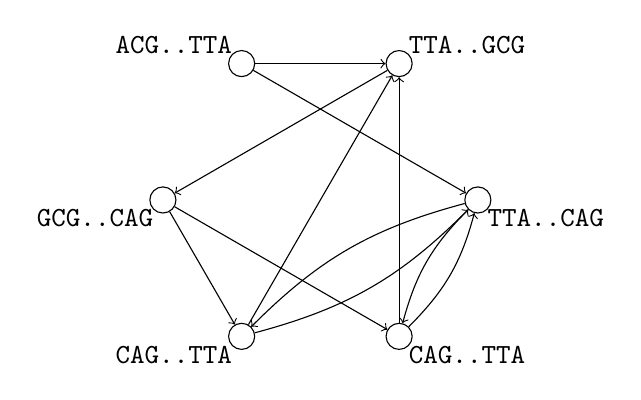
\begin{tikzpicture}
        \node[circle, draw] (1) at (0  :2) {};
        \node[anchor=north west]at (0  :2) {\texttt{TTA..CAG}};
        \node[circle, draw] (2) at (60 :2) {};
        \node[anchor=south west]at (60 :2) {\texttt{TTA..GCG}};
        \node[circle, draw] (3) at (120:2) {};
        \node[anchor=south east]at (120:2) {\texttt{ACG..TTA}};
        \node[circle, draw] (4) at (180:2) {};
        \node[anchor=north east]at (180:2) {\texttt{GCG..CAG}};
        \node[circle, draw] (5) at (240:2) {};
        \node[anchor=north east]at (240:2) {\texttt{CAG..TTA}};
        \node[circle, draw] (6) at (300:2) {};
        \node[anchor=north west]at (300:2) {\texttt{CAG..TTA}};

        \draw[->] (1) to [bend right=15] (5);
        \draw[->] (5) to [bend right=15] (1);

        \draw[->] (1) to [bend right=15] (6);
        \draw[->] (6) to [bend right=15] (1);

        \draw[->] (2) to (4);

        \draw[->] (3) to (2);
        \draw[->] (3) to (1);

        \draw[->] (4) to (6);
        \draw[->] (4) to (5);

        \draw[->] (5) to (2);
        \draw[->] (6) to (2);
      \end{tikzpicture}
      \end{center}
      \captionof{figure}{Exemple de réduction de séquencage ADN vers Chemin
      hamiltonien}

    \subsection{La machine de Turing}

      \subsubsection{Définition}

      Une définition formelle des machines de Turing :

        $(Q, A, B, Q_0, Q_f, T)$

      avec : $Q_0 \subseteq Q, Q_f \subseteq Q, T = Q \times (B \times \left\{\leftarrow, I, \rightarrow\right\} \times B)^k \times Q$

      \begin{itemize}
        \item $Q$ :\'Etats
        \item $A$ :Alphabet d'entré
        \item $B$ :Alphabet de travail
        \item $Q_0$ :\'Etats initia
        \item $Q_f$ :\'Etats finals
        \item $T$ : Transition (k nombre de bandes)
      \end{itemize}

      Exemple :

      \begin{figure}[!htb]
  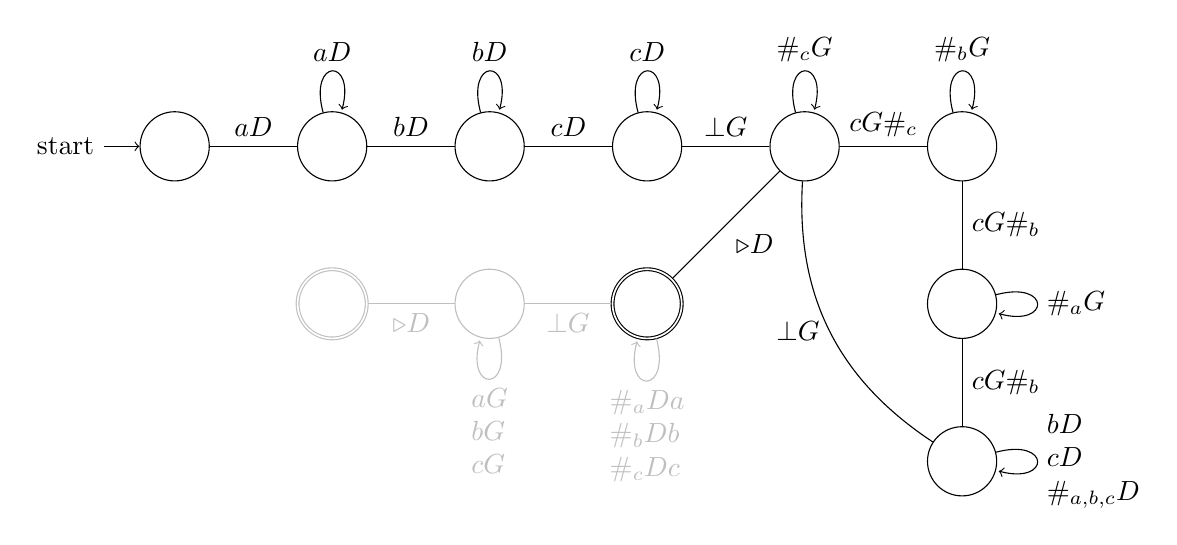
\begin{tikzpicture}
    \node[initial, state] (q0) at (0, 0) {};
    \node[state] (q1) at (2, 0) {};
    \node[state] (q2) at (4, 0) {};
    \node[state] (q3) at (6, 0) {};
    \node[state] (q4) at (8, 0) {};
    \node[state] (q5) at (10, 0) {};
    \node[state] (q6) at (10, -2) {};
    \node[state] (q7) at (10, -4) {};
    \node[state, accepting] (q8) at (6, -2) {}; 
    \node[state, color=lightgray] (q9) at (4, -2) {};
    \node[state, color=lightgray, accepting] (q10) at (2, -2) {};

    \draw (q0) edge[above] node{$aD$} (q1)
          (q1) edge[above] node{$bD$} (q2)
          (q2) edge[above] node{$cD$} (q3)
          (q3) edge[above] node{$\bot G$} (q4)
          (q4) edge[above] node{$cG\#_c$} (q5)
          (q5) edge[right] node{$cG\#_b$} (q6)
          (q6) edge[right] node{$cG\#_b$} (q7)
          (q1) edge[loop above, above] node{$aD$} (q1)
          (q2) edge[loop above, above] node{$bD$} (q2)
          (q3) edge[loop above, above] node{$cD$} (q3)
          (q4) edge[loop above, above] node{$\#_cG$} (q4)
          (q5) edge[loop above, above] node{$\#_bG$} (q5)
          (q6) edge[loop right, right] node{$\#_aG$} (q6)
          (q7) edge[loop right, right, align=left] 
                node {$bD$\\$cD$\\$\#_{a, b, c} D$} (q7)
          (q7) edge[bend left, left] node{$\bot G$} (q4)
          (q4) edge[below right] node {$\triangleright D$} (q8)

          (q8) edge[loop below, below, align=left, color=lightgray] 
                node{$\#_aDa$\\$\#_bDb$\\$\#_cDc$} (q8)
          (q8) edge[below, color=lightgray] node{$\bot G$} (q9)
          (q9) edge[loop below, below, color=lightgray, align=left] 
                node{$aG$\\$bG$\\$cG$} (q9)
          (q9) edge[below, color=lightgray] node {$\triangleright D$} (q10)
          ;
  \end{tikzpicture}
  \caption{Machine de Turing reconnaissant $\left\{a^nb^nc^n| n \geq 1\right\}$}
  \end{figure}

  On peut exécuter cette machine sur une ou plusieurs bandes infinies ou
  bi-infinies, comme celle-ci :

  \begin{tabular}{|c|c|c|c|c|c|c|c|c|c|c}
    \hline
    $\triangleright$ & a & a & a & b & b & b & c & c & c & \ldots\\ 
    \hline
  \end{tabular}



      \subsubsection{Classe P}

      La classe P est l’ensemble des problèmes qui peuvent être
      résolus par des Machines de Turing en temps polynomial
      $\text{\textit{poly}}(n)$.

    \subsection{Classe NP}

      \subsubsection{Définition formelle}

      Un problème de décision appartient à NP s'il existe une relation binaire
      polynomiale $R$ et un polynôme tel que :

      $$ I \in D^+ \Leftrightarrow \exists x, R(I, x) \and |x| \leq p(|I|)$$

      Remarque : $I$ est une instance positive et $R$ est calculable en temp
      polynomial par une machine de Turing.

      \subsubsection{P et NP}

      On peut facilement montrer que $P \subseteq NP$ (il suffit de lancer
      l'algorithme polynomial sur l'entrée).

      Par contre, nous ne savons toujours pas si $NP$ est inclus dans $P$. C'est
      un problème ouvert depuis très longtemps ($1.000.000 \$ $).

      On ferra donc la conjecture suivante : $P \not = NP$.

      \subsubsection{Exemples, Problème du stable}

      \underline{Données} :
      \begin{itemize}
        \item $G = (V, E)$ un graphe
        \item $k \in \mathbb N$ une constante.
      \end{itemize}
      \underline{Question} : Existe-t-il un stable $S$ tel que :
      \begin{itemize}
        \item $S \subseteq V$ avec $|S| \leq k$
        \item $\forall u, v \in S, \{u, v\} \not \in E$
      \end{itemize}

      Stable est bien dans $NP$, il est facile de vérifier qu'un ensemble $S$
      est bien de cardinal plus petit que $k$, et qu'il n'y est pas d'arrête
      dans $E$ qui relit deux éléments de $S$.

    \subsection{Réduction Polynomiale}

      \subsubsection{Principe}

      Problème de la clique : \\
      \underline{Données} :
      \begin{itemize}
        \item $G = (V, E)$ un graphe
        \item $k \in \mathbb N$
      \end{itemize}
      \underline{Question} : Existe-t-il une clique $S$ telle que :
      \begin{itemize}
        \item $S \subseteq V$ avec $|S| \leq k$
        \item $\forall u, v \in S, \{u, v\} \in E$
      \end{itemize}

      On peut résoudre clique à l'aide de stable :

      \begin{center}
      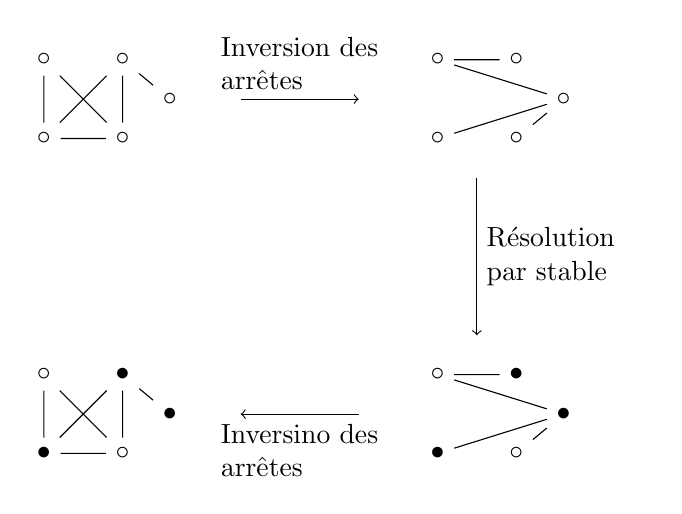
\begin{tikzpicture}
        \node (a) at (0, 0) {$\circ$};
        \node (b) at (1, 0) {$\circ$};
        \node (c) at (1, -1) {$\circ$};
        \node (d) at (0, -1) {$\circ$};
        \node (e) at (1.6, -0.5) {$\circ$};

        \draw (a) -- (d) -- (c) -- (b) -- (d);
        \draw (a) -- (c) (b) -- (e);

        \node (a) at (5, 0) {$\circ$};
        \node (b) at (6, 0) {$\circ$};
        \node (c) at (6, -1) {$\circ$};
        \node (d) at (5, -1) {$\circ$};
        \node (e) at (6.6, -0.5) {$\circ$};

        \draw (a) -- (b) (a) -- (e) -- (d) (e) -- (c);

        \node (a) at (5, -4) {$\circ$};
        \node (b) at (6, -4) {$\bullet$};
        \node (c) at (6, -5) {$\circ$};
        \node (d) at (5, -5) {$\bullet$};
        \node (e) at (6.6, -4.5) {$\bullet$};

        \draw (a) -- (b) (a) -- (e) -- (d) (e) -- (c);

        \node (a) at (0, -4) {$\circ$};
        \node (b) at (1, -4) {$\bullet$};
        \node (c) at (1, -5) {$\circ$};
        \node (d) at (0, -5) {$\bullet$};
        \node (e) at (1.6, -4.5) {$\bullet$};

        \draw (a) -- (d) -- (c) -- (b) -- (d);
        \draw (a) -- (c) (b) -- (e);

        \draw[->] (2.5, -0.5) to node[above, text width=2cm] {Inversion des arrêtes} (4, -0.5);
        \draw[->] (5.5, -1.5) to node[right, text width=2cm]
          {Résolution par stable} (5.5, -3.5);
        \draw[->] (4, -4.5) to node[below, text width=2cm]
          {Inversino des arrêtes} (2.5, -4.5);
      \end{tikzpicture}
      \end{center}

      Cet algorithme nous montre que clique peut se résoudre à l'aide d'un
      algorithme par stable en temps polynomial (si stable est polynomial). On
      appelle ça une réduction polynomiale.

      Soit $D_1 = (D_1^+, D_1^-)$ et $D_2 = (D_2^+, D_2^-)$ deux problèmes de
      décision. On dit que $D_1$ se réduit à $D_2$ sous une réduction de Karp
      $D_1 \leq_K D_2$ s'il existe une fonction $f: D_1 \to D_2$ telle que :
      \begin{itemize}
        \item $I \in D_1^+ \Leftrightarrow f(I) \in D_2^+$
        \item $f$ est calculable en temps polynomial.
      \end{itemize}

      \subsubsection{NP-Complétude}

      Un problème $D$ est $NP$-difficile si $D' \leq D, \forall D' \in NP$ \\
      Un problème $D$ est $NP$-complet si $D$ est $NP$-difficile et $D \in NP$

      \underline{Théorèmes}:
      \begin{itemize}
        \item Si $D \leq D'$ et $D' \leq D''$ alors $D \leq D''$
        \item Si $D$ est $NP$-difficile et $D \in P$ alors $P = NP$
        \item Si $D$ est $NP$-complet alors $D \in P$ ssi $P = NP$
      \end{itemize}

      \subsubsection{Le problème SAT}

      Entrée : une formule sous Forme Normale Conjonctive
      \begin{itemize}
        \item Un ensemble $U$ de variables
        \item Une collection $C$ de clauses disjonctives de littéraux où les
          littéraux sont une variable ou la négation d'une variable.
      \end{itemize}
      Question : Existe-t-il une affection de valeurs aux variables telle que
      toutes les clauses soient satisfaites ?

      \underline{Théorème de Cook-Levin, 1977} : SAT est $NP$-complet

      \subsubsection{SAT $\leq$ Stable}

        On sait que Stable est déjà un problème $NP$, on veut montrer qu'il est
        $NP$-difficile. On va donc faire une réduction polynômial de SAT vert
        stable (SAT $\leq$ Stable).

        \underline{Algorithme} :

        \begin{enumerate}
          \item On crée un sommet pour chaque occurrence de variable dans une
            clause.
          \item On crée des liens entre les sommets d'une même clause.
          \item Enfin on crée des liens entre les variables entre les
            occurrences positive et négative.
        \end{enumerate}

        \underline{Exemple} :

        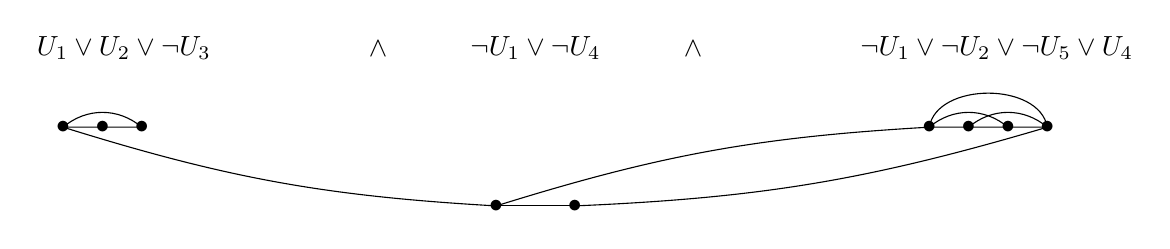
\begin{tikzpicture}
          \node[anchor=east] at (-4, 0) {$U_1 \vee U_2 \vee \neg U_3$};
          \node[anchor=center] at (0, 0) {$\neg U_1 \vee \neg U_4$};
          \node[anchor=west] at (4, 0) {$\neg U_1 \vee \neg U_2 \vee \neg U_5 \vee U_4$};

          \node at (-2, 0) {$\wedge$};
          \node at (2, 0) {$\wedge$};

          \node (u11) at (-6, -1) {$\bullet$};
          \node (u12) at (-5.5, -1) {$\bullet$};
          \node (u13) at (-5, -1) {$\bullet$};

          \node (u21) at (-0.5, -2) {$\bullet$};
          \node (u24) at (0.5, -2) {$\bullet$};

          \node (u31) at (5, -1) {$\bullet$};
          \node (u32) at (5.5, -1) {$\bullet$};
          \node (u35) at (6, -1) {$\bullet$};
          \node (u34) at (6.5, -1) {$\bullet$};

          \draw (u11.center) -- (u12.center) -- (u13.center)
                to[bend right=40] (u11.center);

          \draw (u21.center) -- (u24.center);

          \draw (u31.center) -- (u32.center) -- (u35.center) -- (u34.center)
                to[bend right=40] (u32.center);
          \draw (u31.center) to[bend left=40] (u35.center);
          \draw (u31.center) to[bend left=80] (u34.center);

          \draw (u11.center) to[bend right=7] (u21.center);
          \draw (u21.center) to[bend left=7] (u31.center);
          \draw (u24.center) to[bend right=7] (u34.center);

        \end{tikzpicture}

        \underline{Preuve} :

          \begin{itemize}
            \item SAT $\Rightarrow$ stable de taille $k$ ou plus
              \begin{itemize}
                \item Chaque clause est salifiable
                \item On peut construire un stable de taille $k$ en
                  sélectionnant les littéraux vrais dans chaque clauses.
              \end{itemize}
            \item Stable de taille $k$ ou plus $\Rightarrow$ SAT
              \begin{itemize}
                \item Chaque sommet du stable correspond à un littéral satifiant
                  une clause différentes (étape 2 de l'algo).
                \item Par construction, le stable ne contient pas deux sommets
                  dont l'un correspond à une variable et à sa négation (étape 3
                  de l'algo).
              \end{itemize}
          \end{itemize}

      \subsubsection{SAT $\leq$ D-HAM}

        Voir schéma compliqué fait
        \href{https://gitlab.com/valoranM/latex_diagram/-/blob/main/Problem_reduction/Sat_to_Hamming/ham.pdf?ref_type=heads}{ici}

    \subsection{Retour sur le Séquençage}

      Notre problème de raboutage ADN est donc compliqué ($NP$, la preuve de
      $NP$-difficile est facile à faire).

      On veut une solution qui a ``plus de sens'' du point de vue de la
      biologie. Pour cella, on va rajouter des poids aux arrêts pour avoir des
      variations selon le temps de ressemblance sur le bout de l'ADN. On ne
      pourra plus utiliser les cycles hamiltonien, car il ne prend pas en compte
      les poids, à la place, on se basera sur le problème du voyageur de
      commerce.

  \section{Voyageur de commerce}

    \subsection{Présentation du problème}

      Problème sur les graphes :

        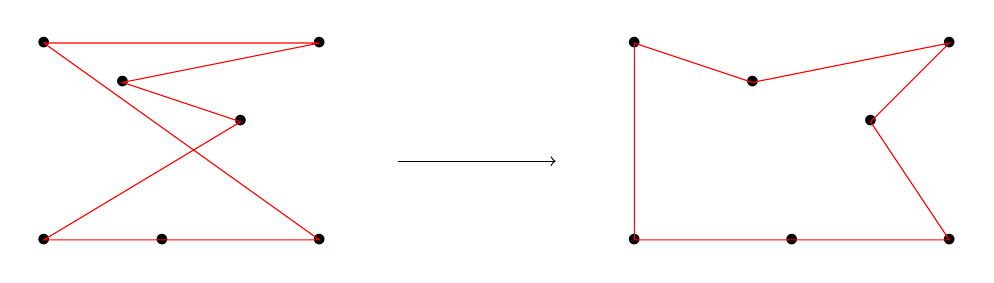
\begin{tikzpicture}
          \node (a) at (4,   0.5) {$\bullet$};
          \node (b) at (4,    -2) {$\bullet$};
          \node (c) at (2,    -2) {$\bullet$};
          \node (d) at (3,  -0.5) {$\bullet$};
          \node (e) at (0.5, 0.5) {$\bullet$};
          \node (f) at (1.5,   0) {$\bullet$};
          \node (g) at (0.5,  -2) {$\bullet$};

          \draw[red] (e.center) -- (a.center) -- (f.center) -- (d.center) -- 
                     (g.center) -- (c.center) -- (b.center) -- (e.center);

          \draw[->] (5, -1) -- (7, -1);

          \node (a) at (8, 0.5) {$\bullet$};
          \node (b) at (9.5, 0) {$\bullet$};
          \node (c) at (12, 0.5) {$\bullet$};
          \node (d) at (11, -0.5) {$\bullet$};
          \node (e) at (12, -2) {$\bullet$};
          \node (f) at (10, -2) {$\bullet$};
          \node (g) at (8, -2) {$\bullet$};

          \draw[red] (a.center) -- (b.center) -- (c.center) -- (d.center) --
                     (e.center) -- (f.center) -- (g.center) -- (a.center);
        \end{tikzpicture}
        \captionof{figure}{Exemple problème Voyageur de commerce}

        \underline{Données} :
          \begin{itemize}
            \item $G=(V, E)$, complet
            \item $\omega : E \to \mathbb{N}$, respecte l'inégalité triangulaire
            \item $K \in \mathbb{N}$
          \end{itemize}

        \underline{Question} :
            Existe-t-il un cycle hamiltonien de poids plut petit que $K$
        \vspace{5mm}

        \underline{Résolution ?} :
          \begin{itemize}
            \item Méthodes exactes telles que le branch and bound
            \item Heuristiques (polynomiales)
          \end{itemize}

    \subsection{Digressions nécessaires}


      \subsubsection{Arbres couvrants de poids minimum}

        \underline{Données}
        \begin{itemize}
          \item Un graphe non orienté $G = (V, E)$
          \item $\omega : E \to \mathbb{N}$, pondération sur les arrêtes
        \end{itemize}

        \underline{Questions} :
            Construire un arbre contenant tous les sommets de $V$ dont le poids
            minimum est minimum. Le poids d'un arbre étant la somme des poids de
            ces arrêtes

      \subsubsection{Graphe eulérien}

          Un cycle est \underline{eulérien} est un cycle passant une et une seule fois par
          chaque arrête d'un graphe. Un graphe est eulérien s'il admet un tel
          cycle.\\
          Un \underline{graphe est eulérien} ssi le degré de chaque sommet est pair.

      \subsubsection{Couplage (Matching)}

          Un \underline{couplage} d'un graphe $G = (V, E)$ est un sous-ensemble d'arêtes $M
          \subseteq E$ tel que $\forall a, b \in M$, $a$ et $b$ n'ont pas de
          sommets en commun.\\
          Un \underline{couplage est parfait} si tous les sommets du graphe
          sont couverts par le couplage

      \subsubsection{Set Cover}
 
        \underline{Données}
          \begin{itemize}
            \item $E$ un ensemble d'éléments
            \item $S$ une famille de sous ensembles de $E$
            \item $K \in \mathbb{N}$
          \end{itemize}

          \underline{Questions} : Existe-t-il un sous ensemble $C$ de $S$
                                  de taille plus petit que $K$ tel-que l'union
                                  de tous les éléments de $C$ soit égale à $E$

    \subsection{Approximation}

    \subsection{Inapproximation}

  \section{Exemple : Centre médical pour des villes}

    \underline{Données} :

      \begin{itemize}
        \item $G = (V, E)$
        \item $\omega : E \to \mathbb{N}$
        \item $D \in \mathbb{N}$, distance maximale (K-Centre)
        \item $K \in \mathbb{N}$, le nombre max de maison (Dominant)
      \end{itemize}

    \underline{Question} : Existe-t-il un ensemble $M \subseteq V$ de centre
                           tel-que toutes les villes soient à une distance
                           plus petite que $D$ d'un centre

    \subsection{K-Centre}

      On cherche à optimiser la distance (de gauche).

      Trouver $M \subseteq V, |M| \leq K$ et
      $\max_{v\in V} \min_{m \in M} d(v, m)$ est minimum

    \subsection{Dominant ``à peu près''}

      On cherche à minimiser la distance (de droite).

      Trouver $M \subseteq, \forall v \in V, \min_{m \in M}(v, m) \leq D$
      et $|M|$ est minimum


  \section{Métaheuristique}

    \subsection{Introduction}

      \define Heuristiques : 

    \subsection{Métaheuristiques à parcours}

    \subsection{Métaheurisitiques à population}

    \subsection{\'Evaluation de la performance d'une heuristique}

\end{document}
